\documentclass{beamer}
\usetheme{default}
\usecolortheme{crane}
\usepackage{amsmath}
\usepackage{amsfonts}
\usepackage{epstopdf}
\usepackage{amssymb}
\usepackage{graphicx}
\usepackage{movie15}
%\usepackage{CJKutf8}
\title{OpenLCDFDM: an finite-difference LCD simulator}
\author{\texorpdfstring{Zong-han, Xie\newline\url{icbm0926@gmail.com}}{Zong-han, Xie}}
\date{\today}
\begin{document}
%\begin{CJK}{UTF8}{cwmc}
\begin{frame}
\titlepage
\end{frame}
\begin{frame}[label=licensepage]
\frametitle{License of this slide}
Introduction to Fourier transform and signal analysis by Zong-han, Xie (\href{icbm0926@gmail.com}{icbm0926@gmail.com}) is licensed under a Creative Commons Attribution-NonCommercial 4.0 International License. \newline
\begin{center}
\includegraphics[scale=2]{by-nc-sa.eps}
\end{center}
\end{frame}
\AtBeginSection[]
{
  \begin{frame}
    \frametitle{Outline}
    \tableofcontents[currentsection]
  \end{frame}
}

\begin{frame}
\frametitle{LCD on consumer products}
\begin{center}
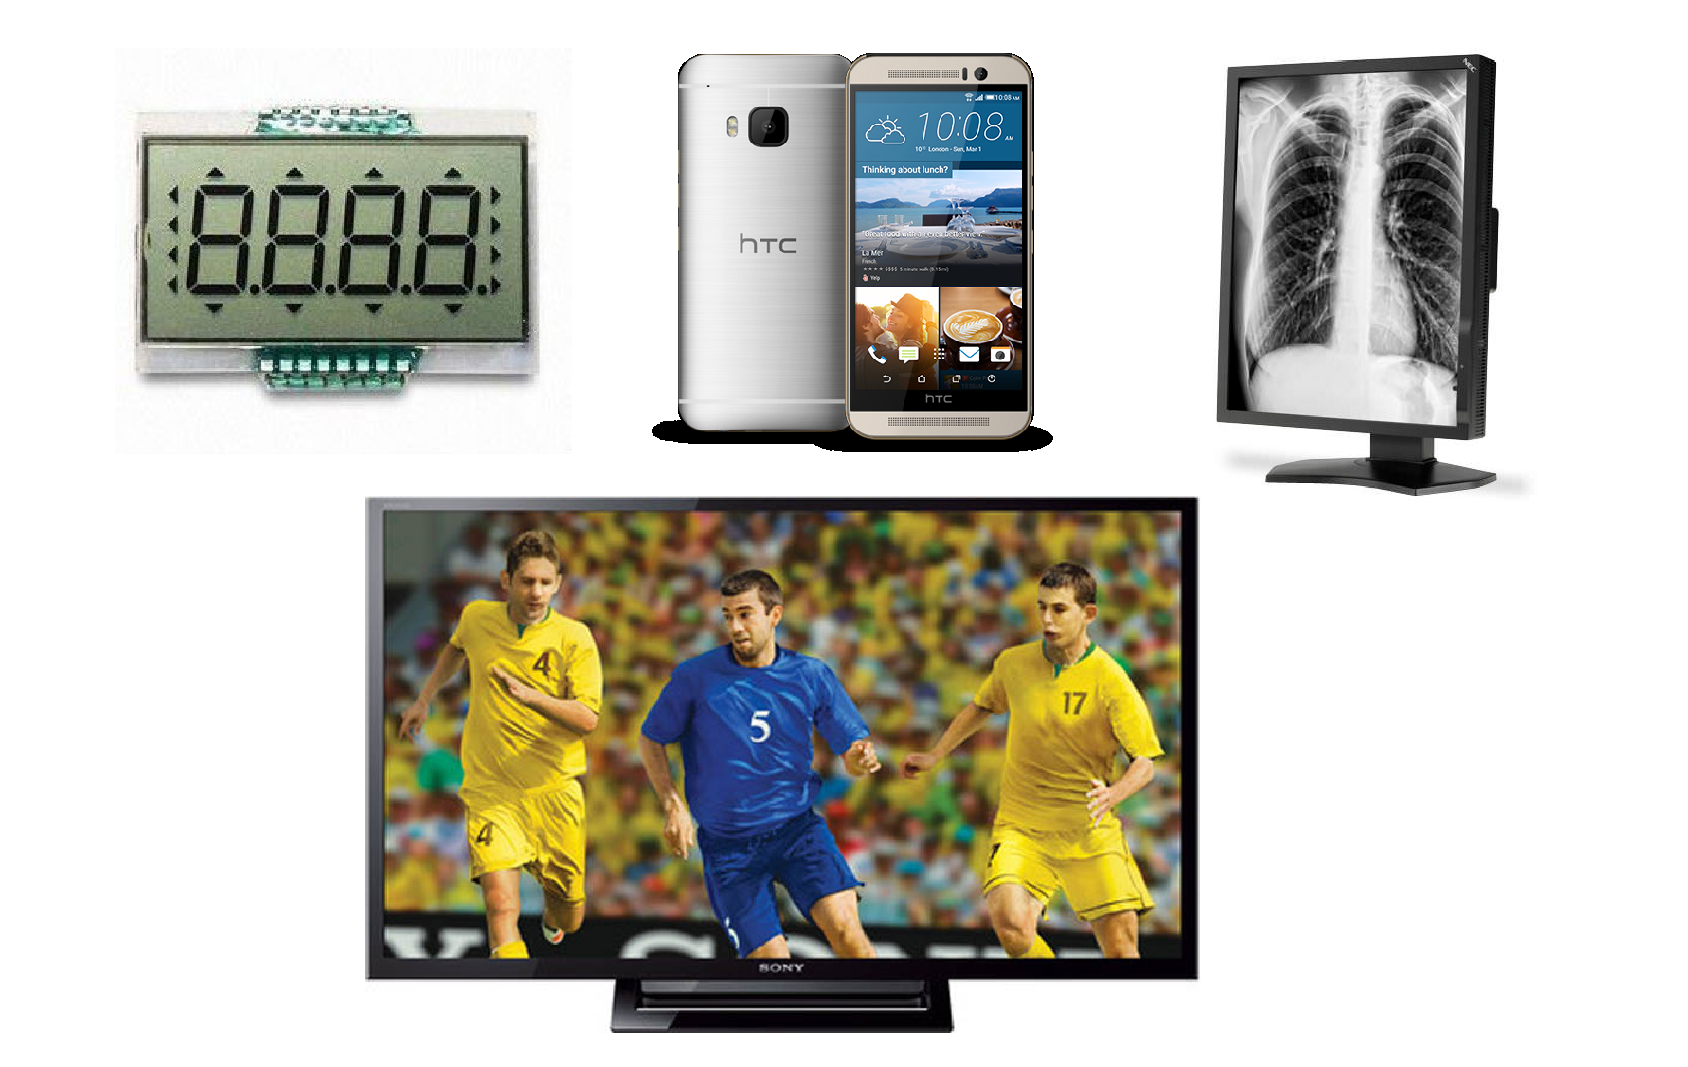
\includegraphics[scale=0.4]{LCD_Consumers.eps}
\end{center}
\end{frame}
\begin{frame}
\frametitle{LCD display structure}
\begin{center}
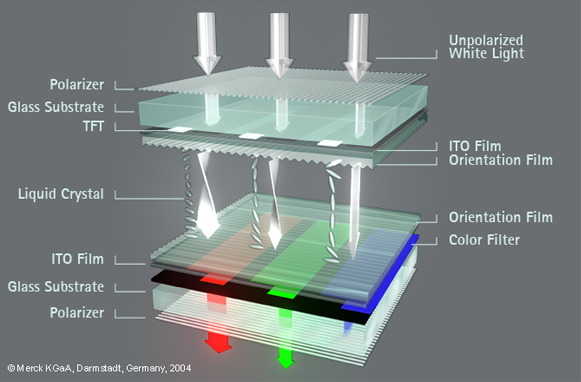
\includegraphics[scale=0.4]{LCD_Infografik_ENG_580_tcm1113_40163.jpg}
\\
Liquid crystal layer is served as an optical switch, it determines how much light from light source (backlight in LCD display) can propagate through.
\end{center}
\end{frame}
\begin{frame}
\frametitle{Polarization}
\begin{center}
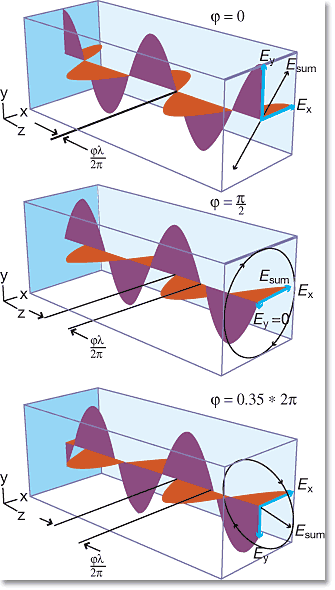
\includegraphics[scale=0.4]{polarization.png}
\end{center}
\end{frame}
\begin{frame}
\frametitle{Birefringence and phase retardation}
If a material has anisotropic refractive index, it is called a birefringence material. It causes different light speed on different polarization. It canges phase diefference between
two polarization of light, it's called phase retardation.
\begin{center}
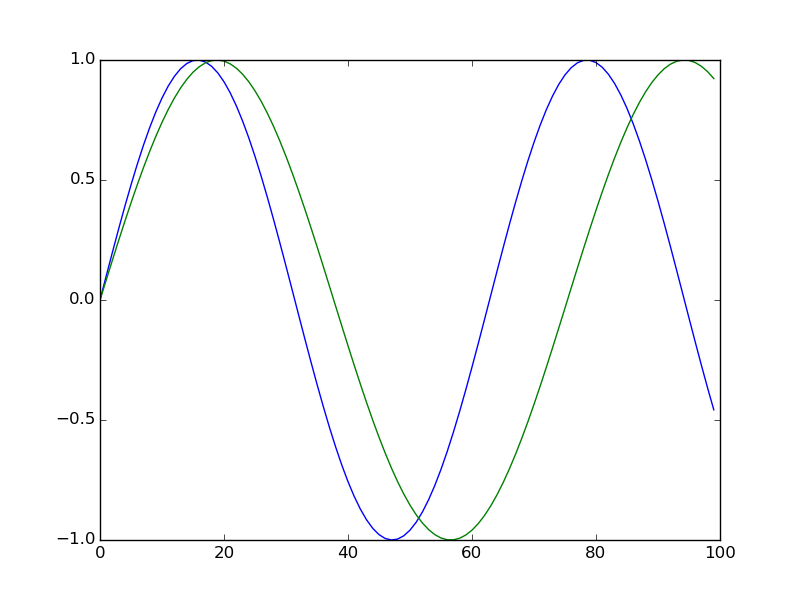
\includegraphics[scale=0.4]{retardation.png}
\end{center}
\end{frame}
\begin{frame}
\frametitle{Electric controlled birefringence}
\begin{center}
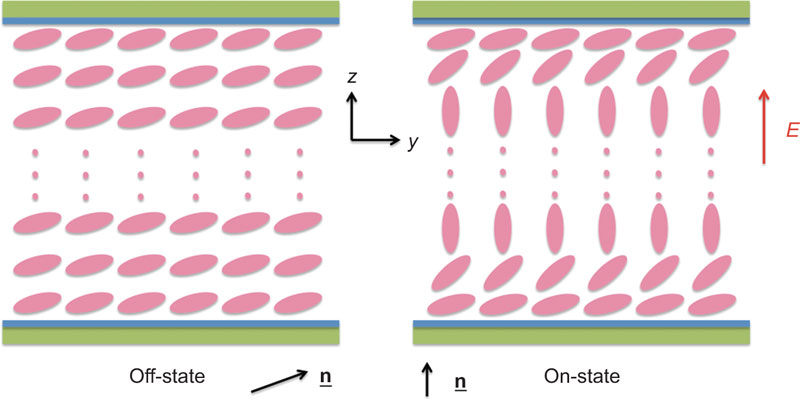
\includegraphics[scale=0.4]{ECB.jpg}
\end{center}
Due to the anisotropic dielectric property of liquid crystal, when external electric field is applied, the LC molecule will start to align with the electric field.
\end{frame}
\begin{frame}
\frametitle{Calculation models}
\begin{itemize}
\item<1-> Find LC distribution:
\begin{itemize}
\item<1-> Continuum theory for liquid crystal
\item<1-> Laplace equation in anisotropic media
\end{itemize}
\item<1-> Optical calculation: Extended Jones matrix method
\end{itemize}
\end{frame}
\begin{frame}
\frametitle{Continuum theory for liquid crystal}
Using Oseen-frank elastic free energy density to model the elastic property of liquid crystal molecules.
The LC molecule distriution is acquired by minimizing the total energy density which includes elastic free energy density and electric field energy density.
\begin{eqnarray}
f(\vec x) &=& \frac{1}{2}K_{11}(\nabla\cdot\vec n)^2+\frac{1}{2}K_{22}(\vec n\cdot\nabla\times\vec n)^2 + \frac{1}{2}K_{22}(\vec n\times\nabla\times\vec n)^2\nonumber \\
&&+q_0K_{22}(\vec n\cdot\nabla\times\vec n) - \frac{1}{2}K_{22}(\vec D\times\vec E)\nonumber
\label{eq:free_energy}
\end{eqnarray}
where $\vec D = \epsilon(\vec x)\cdot \vec E$ and $\epsilon(\vec x)$ is a 3X3 dielectric tensor. $\vec n$ is a unit vector for local liquid crystal orientation.
\end{frame}
\begin{frame}
\frametitle{Laplace equation in anisotropic media}
Laplace equation:
\begin{eqnarray}
\nabla \cdot \epsilon(\vec x) \cdot \nabla \phi(\vec x) &=& 0 \nonumber \\
\label{eq:laplace}
\end{eqnarray}
$\epsilon(\vec x)$ is the local dielectric tensor decided by the local oritation of LC molecule. 
\end{frame}
\begin{frame}
\frametitle{Extended Jones matrix method}
Under the assumption that the two refractive index are very close, the original Jones matrix method can be extended to extended Jones matrx method.
\end{frame}
\begin{frame}
\frametitle{OpenLCDFDM program structures}
\end{frame}
\begin{frame}
\frametitle{Demo}
\end{frame}
\begin{frame}
\frametitle{References}
\begin{thebibliography}{0}
%\bibitem{SNGP} Supplementary Notes of General Physics by Jyhpyng Wang, \url{http://idv.sinica.edu.tw/jwang/SNGP/SNGP20090621.pdf}
\end{thebibliography}
\end{frame}

%---------------Examples of Latex---------
%\begin{frame}
%\frametitle{2nd page}
%\begin{block}{block}
%\begin{eqnarray}
%\frac{1}{2}
%\end{eqnarray}
%\end{block}
%\begin{alertblock}{alertblock}
%alertblock content
%\end{alertblock}
%\end{frame}
%\begin{frame}
%\frametitle{3rd page}
%\begin{itemize}
%\item<1-> 第一
%\item<1-> 2nd
%\item<2-> 3rd
%\item<3-> etc.
%\hyperlink{1stpage}{\beamerbutton{ooxx}}
%\end{itemize}
%\end{frame}
%\end{CJK}
\end{document}
